
\chapter{Introduction}
%\addcontentsline{toc}{chapter}{Introduction}


\minitoc

One fundamental goal of Artificial Intelligence (\ai) is to design embodied autonomous interactive agents that can evolve in various environments and complete a wide range of tasks. To that end, researchers in \ai take several angles of attack and rely on different paradigms that consider different drivers for learning. In Reinforcement Learning (\rl)~\citep{sutton2018reinforcement}, agents learn from \textit{exploration} of their environment. They rely solely on their experience of the world in order to solve a pre-defined task. In Imitation Learning (\il)~\citep{pomerleau1991efficient}, agents learn from \textit{demonstrations}, i.e. trajectories provided by an expert that correspond to the transitions required to take to solve a pre-defined task.  In Multi-Agent Reinforcement Learning (\marl)~\citep{LITTMAN1994157}, agents learn in \textit{cooperation} and need to interact with each other in order to solve collaborative tasks.


Recent extensions of \rl algorithm have shown success in solving a wealth of problems such as playing the Atari videogames at super-human levels~\citep{mnih2015human}, beating chess and go world champions~\citep{silver2016mastering}, controlling stratospheric baloons~\citep{bellemare2020autonomous} or even maintaining plasma in fusion reactors~\citep{degrave2022magnetic}. Similarly, \il methods coupled to Transformers~\citep{vaswani2017attention} have enabled the training of a generalist agent on a massive dataset of diverse interactions~\citep{reed2022a}. It has also been used to perform in-context reinforcement learning via algorithm distillation~\citep{laskin2022incontext}. Finally, multi-agent methods have permitted populations of agents to play hide and seek~\citep{Baker2020Emergent} or even to collaboratively solve common-pool resource problems~\citep{perolat2017commonpool}.

But unlike humans, these algorithms are still heavily sample-inefficient, requiring billions of transitions to become proficient on isolated tasks. Most importantly, they lack the ability to generalize and transfer across a wide variety of problems, to be creative, and tackle tasks never seen during training. They are far from displaying human-like capabilities in terms of open-ended learning. This is, perhaps, because they rely on isolated signals for learning. The way forward might be to build on child development theory and to consider learning from \textit{sociocultural interactions}. Indeed humans are social beings, they interact and cooperate with their peers~\citep{tomasello_cultural_1999,tomasello_understanding_2005, brewer2014addressing}. As soon as they discover and learn a language, they assimilate thousands of years of experience embedded in their culture~\citep{bruner1991narrative}.  Most of their skills could not be learned in isolation. Formal education teaches them to reason systematically, books teach them history, and YouTube might teach them how to cook. Most importantly, humans' values, traditions, norms, and most of their goals are cultural in essence.

The present research proposes to immerse artificial agents in social contexts in order to observe the impact of sociocultural interactions on learning. As displayed in figure~\ref{fig:intro_chapter_def}, it has a dual objective. In the first part of this manuscript, we propose to use artificial agents as an anthropological tool to study the formation of cultural conventions in populations of individuals. More specifically, we investigate the key mechanisms required for the self-organization of cultural models between artificial agents in absence of pre-existing conventions. In the second part, we focus on autonomous artificial agents exploiting already existing cultural conventions to augment their capabilities in the open-ended skill acquisition problem. To accomplish this, we build on previous theories at the intersection of developmental psychology and machine learning to introduce a new framework coined \textit{Vygotskian Autotelic Artificial Intelligence} which enables sociocultural interactions to transform agents' learning signal, yielding better learners. 

%
\begin{figure}[!h]
\centering
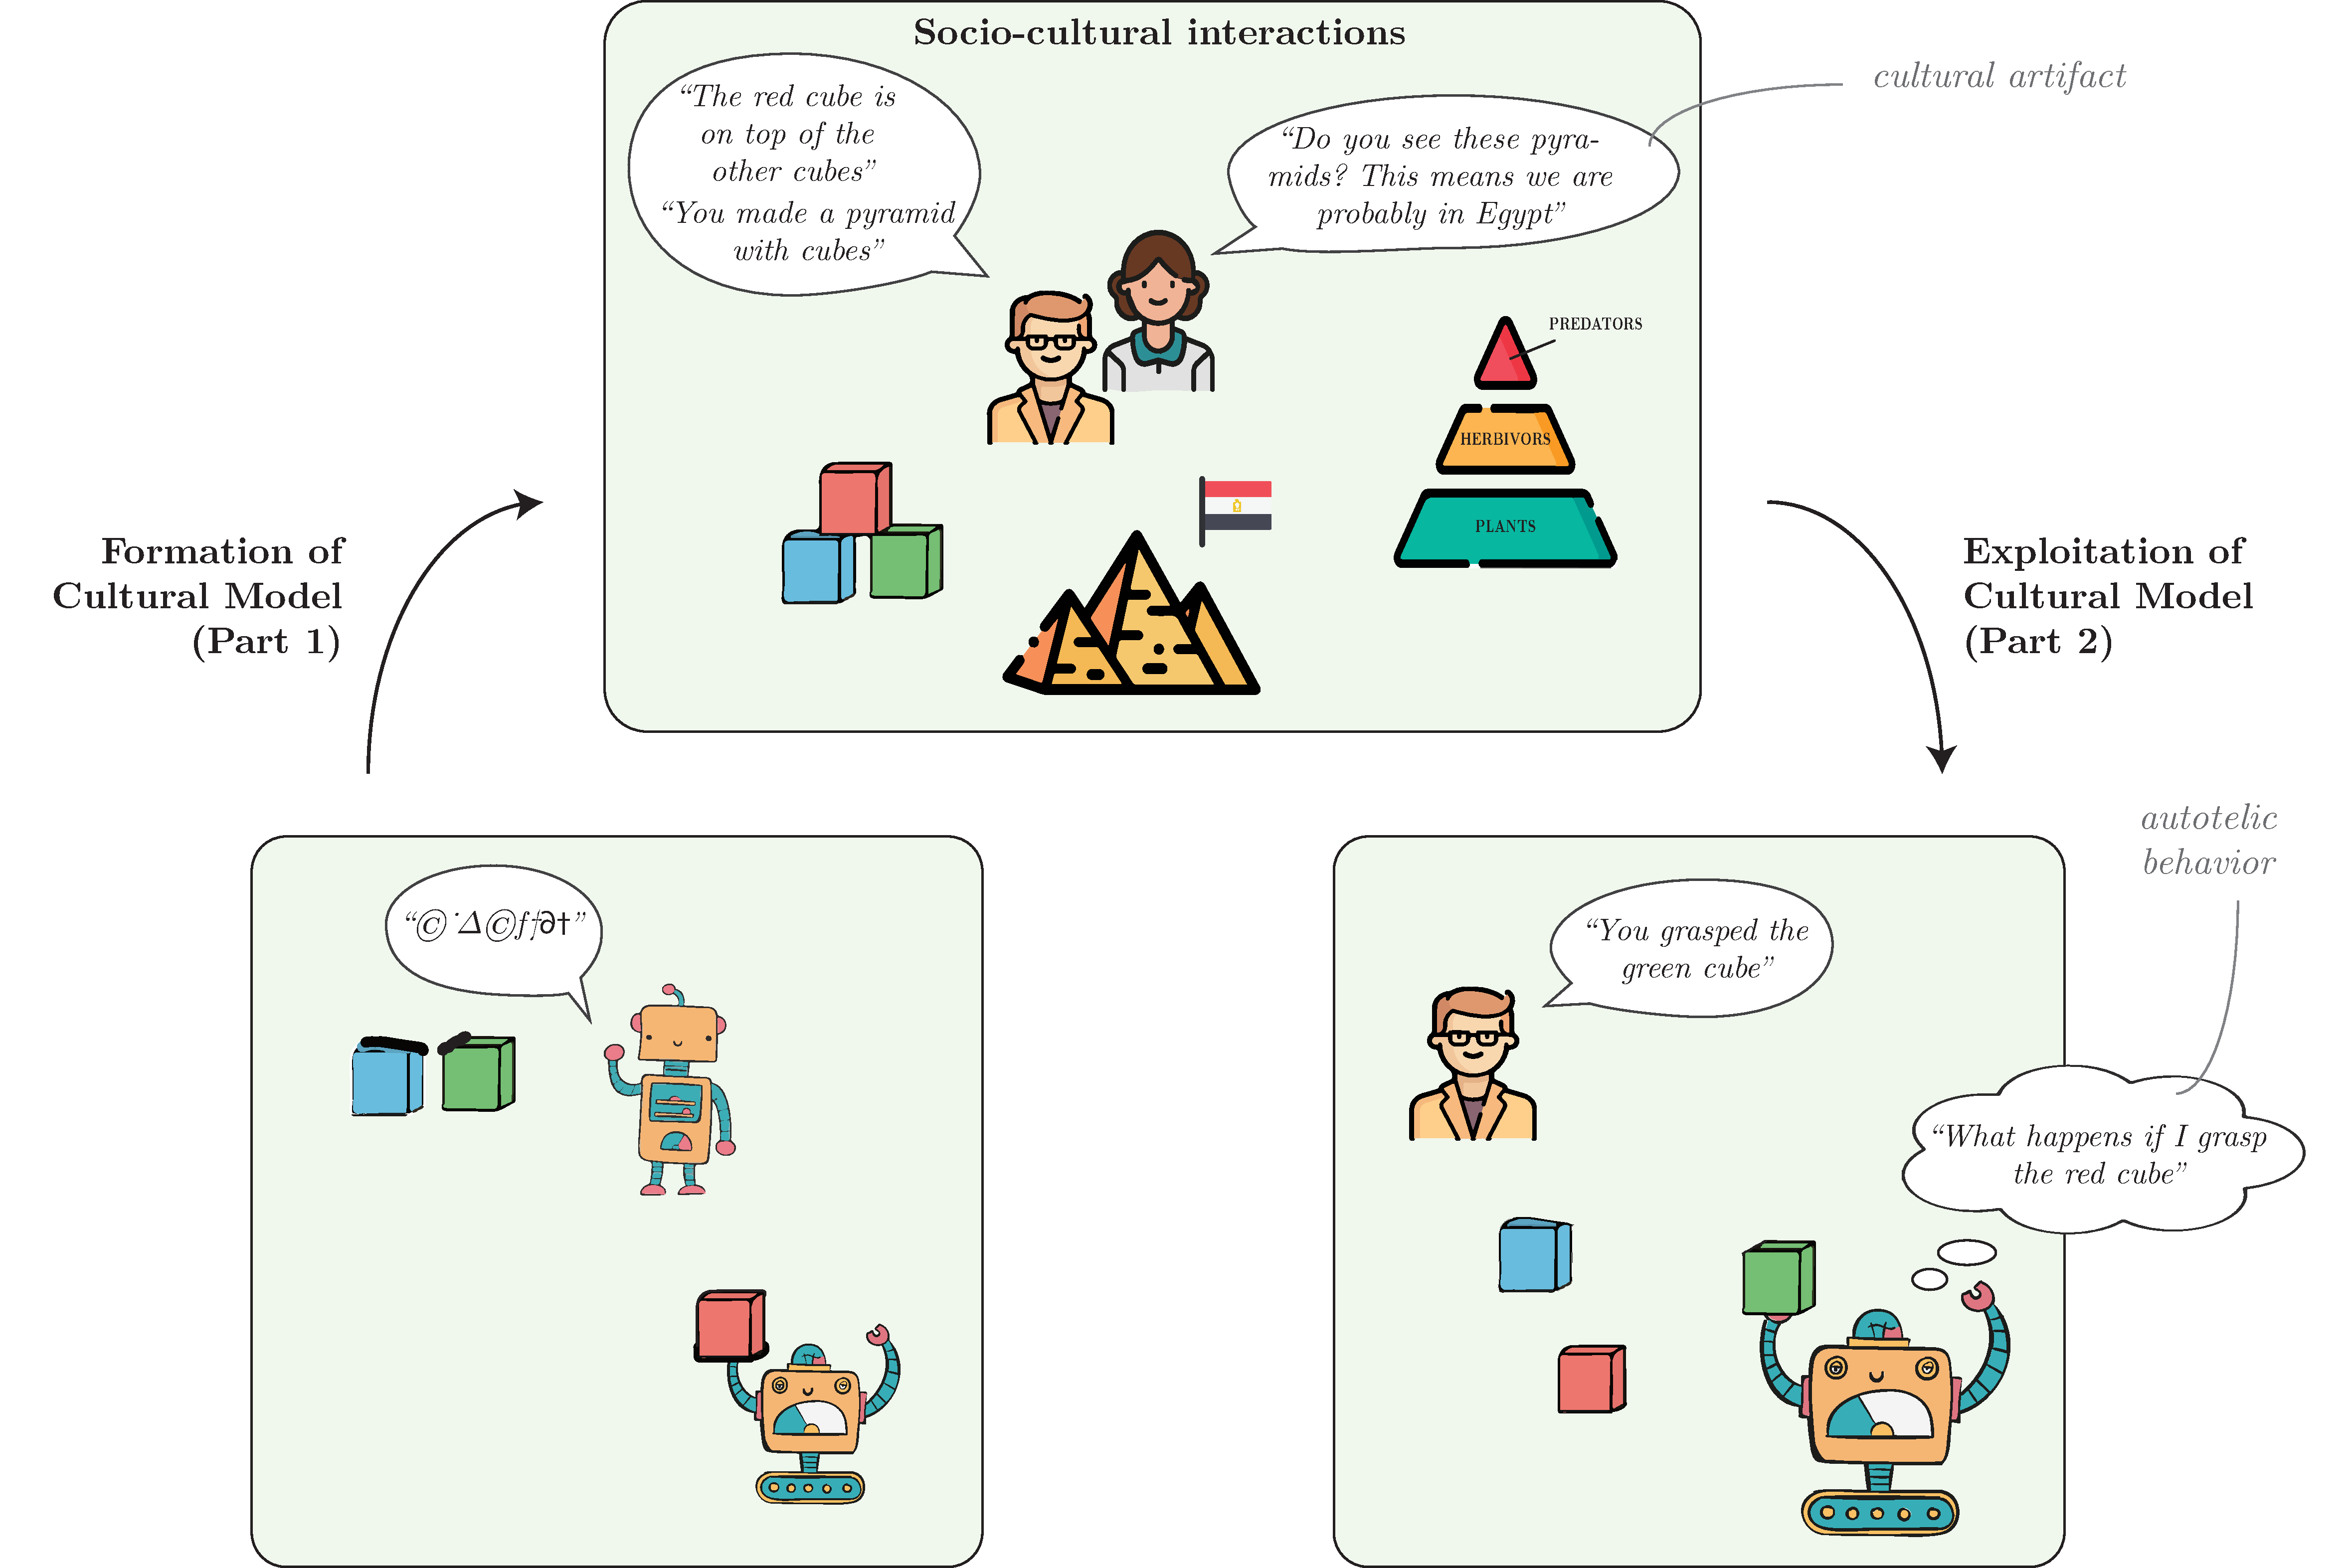
\includegraphics[width=1\textwidth]{intro/intro_chapter_def.pdf}
\caption{\textbf{Dual organization of the present research.} In the first part we take a bottom-up approach and study the self-organization of cultural conventions in artificial agents from social interactions. In the second part, we use a top-down approach to investigate the impact of pre-existing cultural conventions on artificial agents when they interact with social peers.}
\label{fig:intro_chapter_def}
\end{figure}

The remaining of this introduction presents key features of human learning that enable us to define the important notions of "autotelic learning" and "cultural convention" at the center of this research. We then close it with a short intuitive explanation of the position of this research with respect to other paradigms in \ai and a summary of our contributions.


\section{Humans are goal-directed social learners}

Humans are an incredible source of inspiration for \ai. They are the fastest learning system we can ever witness. Within only a few years, children learn to crawl and navigate their home, identify and manipulate objects, they even learn to speak and interact with their peers. How do they reach such a level of proficiency in such a short period of time? 

\subsection{Humans are autotelic learners}

A central aspect of human development is the notion of goal. Studying the use of the notion of goal in past psychological research, \citet{elliot2008goal} propose the following general definition:
\begin{quote}
    "\textit{A goal is a cognitive representation of a future object that the organism is committed to approach or
    avoid}"~\citep{elliot2008goal}.
\end{quote}
%
A goal is therefore a future projection that influences human behaviors. During exploratory play, children constantly invent and pursue their own problems/goals~\citep{chu2020exploratory}. In particular, children's exploration seems to be driven by intrinsically motivated brain processes that trigger spontaneous exploration for the mere purpose of visiting interesting situations~\citep{gopnik1999scientist,kaplan2007search,kidd_psychology_2015}. But how do we measure interestingness?  \citet{hunt1965} propose to evaluate situations in term of \textit{optimal incongruity}. Similarly, \citet{berlyne1966curiosity} suggest relying on the notion of \textit{intermediate level of novelty} while \citet{Kidd2012TheGE} showed that young infants focus on goals with \textit{intermediate complexity}.  Finally, \citet{csikzentmihalyi1997finding}, in his flow theory suggests that for human beings to feel pleasure during learning they should target goals with \textit{optimal challenge}. He uses the term \textit{autotelic} to describe intrinsically motivated agents that are in the flow state. 

\begin{tcolorbox}
\small
\paragraph{Definition}
\gls{Autotelic}: from the Greek \textit{auto} (self) and \textit{telos} (end, goal), characterizes agents that generate their own goals and learning signals. In is equivalent to \textit{intrinsically motivated and goal-conditioned}.
\end{tcolorbox}

\subsection{Humans are social learners}

Social interactions are another crucial property of human development. At birth, humans enter a culture that strongly shapes their development~\citep{whorf_language_1956}. Humans are social beings; intrinsically motivated to interact and cooperate with their peers~\citep{tomasello_cultural_1999,tomasello_understanding_2005, brewer2014addressing}. Indeed, we use social interactions and language at every stage of our development to communicate, cooperate, teach and organize our thoughts. 

\paragraph{Cooperation}

First, social interactions enable us to \textbf{cooperate}, to jointly commit to shared goals. \citet{Tomasello+2019} describes this collaborative behavior as \textit{shared intentionality}. According to him, shared intentionality arises around nine months and enables us to relate to others as equals and to align on low-level common goals such as "looking in the same direction". Shared intentionality allows us to mentally represent and then adopt another's goal. It is thus very linked to the theory of mind~\citep{wellman1992child}. It allows us to share goals, emotions, attention, or even knowledge. As we grow older, shared intentionality becomes \textit{collective intentionality} and allows us to be part of a society in which goals are associated with social norms and conventions. In a recent study, \citet{mcclung2017cooperation} use an egg hunt game to show that group membership and the ability to talk led to increased collaboration between participants. By analyzing the conversation they found that in-group participants were talking about the hunt in terms of a shared or common goal, while out-group participants used individual goals.

\paragraph{Teaching}


In a more structured way, social interactions also enable us to \textbf{teach}. The idea that social interactions provide a structure for teaching has been supported by many researchers including~\citet{vygotsky_play_1933,bruner1985child, rohlfing_alternative_2016,vollmer2016pragmatic}. \citet{bruner1985child} specifically proposed the concept of \textit{pragmatic frames}: patterns of behaviors that are used to achieve a goal and that are developed through repeated and sequential interactions between a teacher and a learner. According to Bruner, pragmatic frames are made of two key components: 1) a \textit{syntax} which is the observable part of the interactions and includes the sensory means (modalities) as well as the role of each actor; 2) a \textit{meaning} which is the learning content. In his book, \citet{bruner1985child} takes the example of the \textit{book-reading frame} during which the teacher points and asks for labels before providing feedback and correcting the learner depending on their answer. In this case, the pointing/asking/answering mechanism is the syntax and the label is the meaning. Pragmatic frames can happen in a variety of modalities but as we just saw with the book-reading frame, they are often multi-modal and imply linguistic interactions.


\begin{wrapfigure}{r}{0.5\textwidth}
\centering
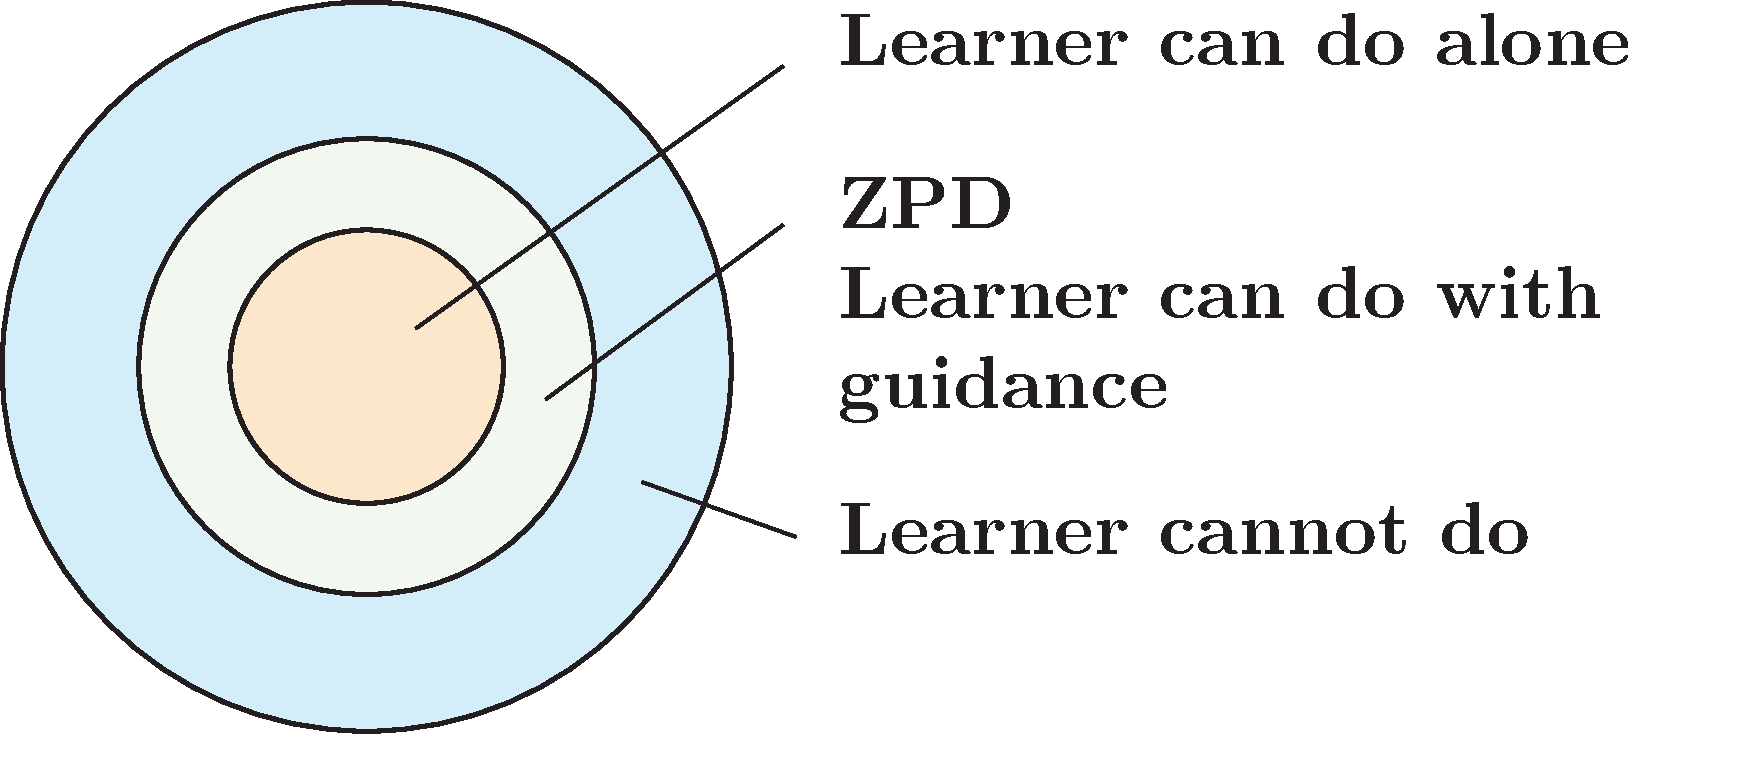
\includegraphics[width=.5\textwidth]{intro/zpd.pdf}
\caption{ZPD Illustration}
\label{fig:intro_zpd}
\end{wrapfigure}
%
Pragmatic frames may also adapt to the learners' abilities. In Vygotsky's \textit{zone of proximal development}~\citep{vygotsky_thought_1934}, caretakers naturally scaffold the learning experiences of children, tailoring them to their current objectives and capacities. Through encouragement, attention guidance, explanations, or plan suggestions, they provide cognitive aids to children in the form of interpersonal social processes. In this zone, children can benefit from these social interactions to achieve more than they could alone as illustrated in figure~\ref{fig:intro_zpd}. In Vygotsky's terms, the \textsc{zpd} is defined as
\begin{quote}
"\textit{the distance between the actual developmental level as determined by independent problem solving and the level of potential development as determined through problem-solving under adult guidance, or in collaboration with more capable peers}"~\citep{vygotsky_thought_1934}	
\end{quote}



\paragraph{Thoughts}

The language we use in social interaction can also be a cognitive tool that facilitates \textbf{thinking}. In Vygotsky's theory, children \textit{internalize} linguistic and social aids and progressively turn these interpersonal processes into intrapersonal \textit{psychological tools}. This essentially consists in building internal models of social partners such that learners can self-generate contextual guidance in the absence of an external one. Social speech is internalized into private speech (an outer speech of children for themselves), which, as it develops, becomes more goal-oriented and provides cognitive aids of the type caretakers would provide~\citep{vygotsky_thought_1934,berk_why_1994}. Progressively, it becomes more efficient and abbreviated, less vocalized, until it is entirely internalized by the child and becomes \textit{inner speech}. This inner speech would enable \textit{thinking in language}~\citep{carruthers1998thinking}. The relation between language and thought in humans is the subject of a great debate and will be discussed in greater detailed in chapter~\ref{chap:foundation_vaai}, section~\ref{sec:language_and_though} when introducing the Vyogtskian Auotelic \ai framework.

\paragraph{Cultural ratchet}

Finally, language is a cultural artefact inherited from previous generations and shared with others. It supports our cultural evolution and allows humans to efficiently transfer knowledge and practices across people and generations~\citep{henrich2003evolution,morgan_experimental_2015,chopra2019first}\,---\,a process known as the \textit{cultural rachet}~\citep{tomasello_cultural_1999}. Through shared cultural artefacts such as narratives, we learn to share common values, customs and social norms, we learn how to navigate the world, what to attend to, how to think, and what to expect from others~\citep{bruner1990acts} 

\paragraph{Cultural Convention}

In light of the various properties of social interactions presented in this section, we introduce the notion of \textit{cultural convention} which generalizes pragmatic frames to internal (intrapersonal) social production. More specifically, we propose the following definition.

\begin{tcolorbox}
\small
\paragraph{Definition}
\gls{Cultural Convention}: Any social production, linguistic or physical, internal or interpersonal, used to communicate, cooperate, teach, think, or transmit.
\end{tcolorbox}

\newpage

\section{Towards Interactive Social Autonomous Agents}

The present research aims at bridging developmental psychology with recent \ai methods used to design embodied artificial agents. Building on the "autotelic" and the "cultural convention" notions, our goal is to build interactive social autotelic agents. For this purpose, we immerse artificial agents in social contexts and equip them with learning mechanisms to either construct cultural conventions (in part~\ref{part:formation}) or to exploit cultural conventions to discover new skilss (in part~\ref{part:exploitation}). 

\begin{figure}[!h]
\centering
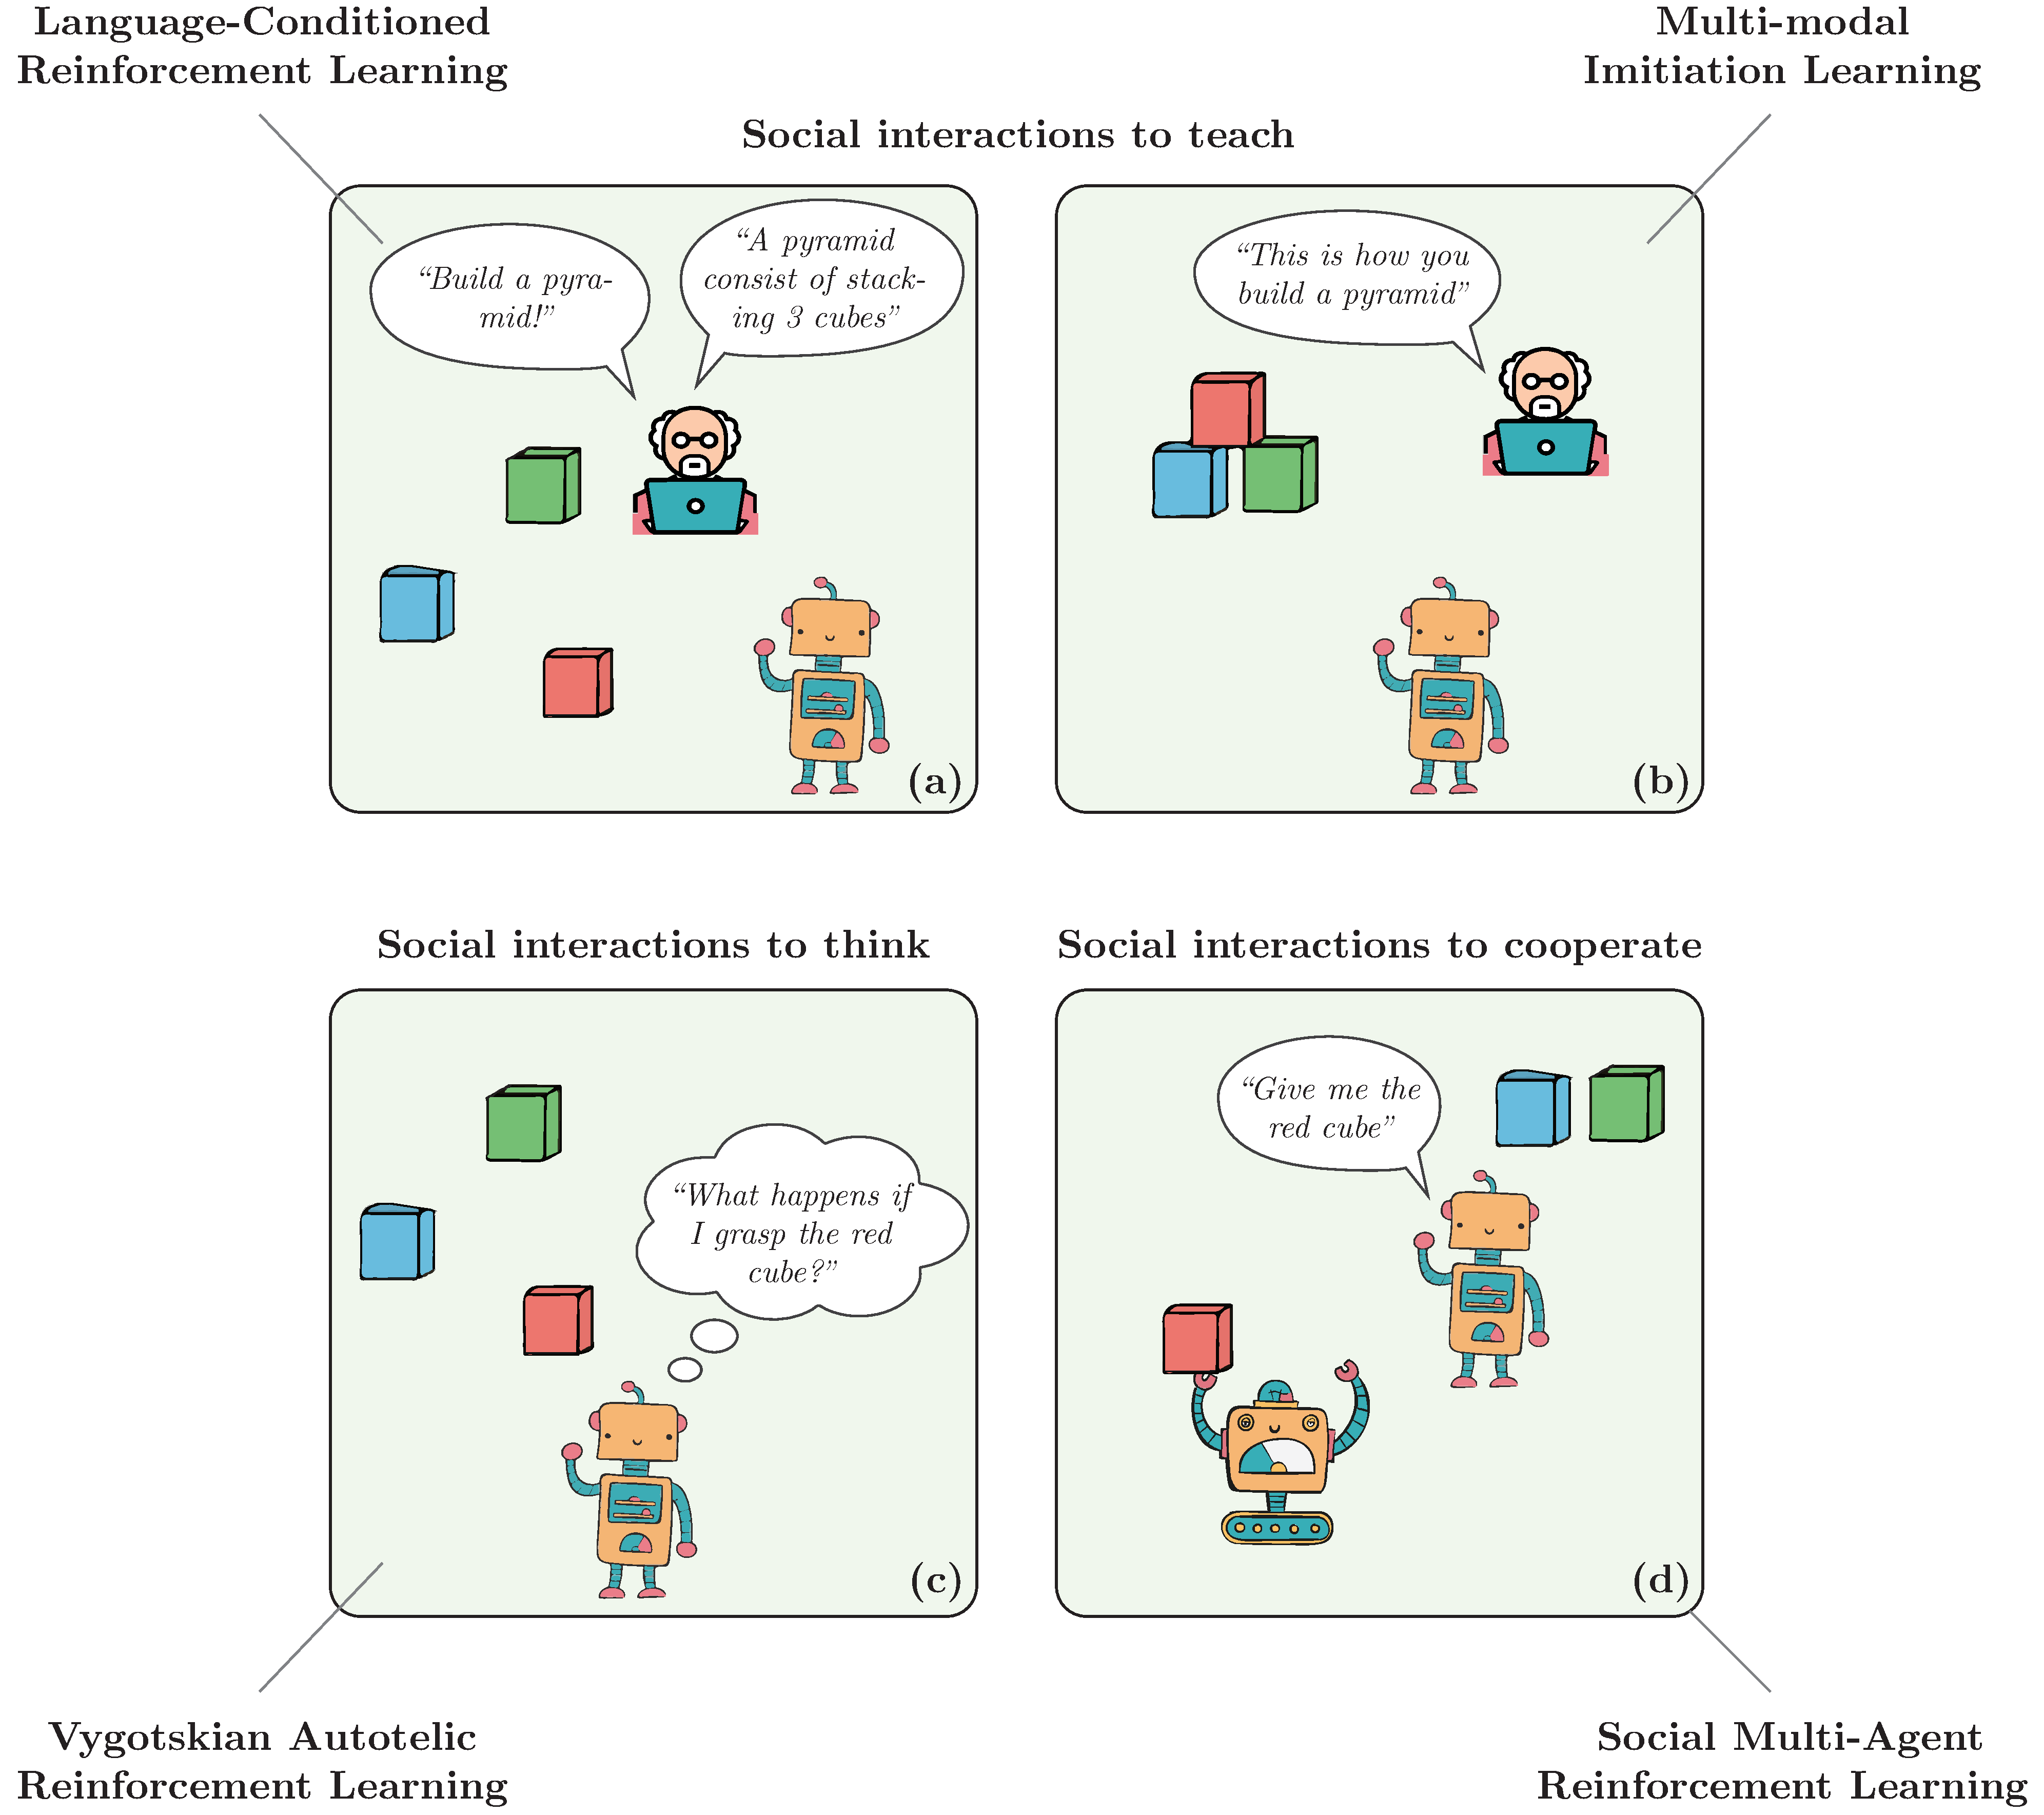
\includegraphics[width=1\textwidth]{intro/language_paradigms.pdf}
\caption{\textbf{Social Interactions in different \ai paradigms.} Social interactions and language instructions are used in both \rl and \il setting to guide learners. Language can also serve as a cognitive tool to represent goals in autotelic learning. Finally, they can help agents communicate and cooperate in \marl.}
\label{fig:intro_language_paradigms}
\end{figure}

The immersion of artificial agents in social worlds does not require starting from fresh grounds. In fact, numerous works already include social elements in pre-existing \ai paradigms. In a recent survey, \citet{Luketina2019} review several approaches instructing Reinforcement Learning agents with language, either to condition them or to assist them as displayed in figure~\ref{fig:intro_language_paradigms}~(a). Similarly, recent imitation learning settings have had their training datasets augmented with linguistic descriptions of expert trajectories~\citep{ALFRED20,pashevich2021episodic} as displayed in figure~\ref{fig:intro_language_paradigms}~(b). In the present research, we will demonstrate that agents can use language as a cognitive tool to imagine creative goals~\citep{colas2022language} as illustrated in figure~\ref{fig:intro_language_paradigms}~(c). Finally, \citet{jaques2019social} recently presented a \marl framework where agents use social motivations to solve collaborative tasks such as the one depicted in figure~\ref{fig:intro_language_paradigms}(d). 

\paragraph{Objectives}

The general objective of the present research is to investigate the two following questions: 
\begin{itemize}
	\item \textbf{How can cultural conventions self-organize when artificial agents interact?} The objective of the first part of this research is to investigate the key mechanisms required for the \textbf{formation} of cultural conventions between artificial agents. In part~\ref{part:formation}, we will specifically consider social interactions between two artificial agents that both integrate learning dynamics. We, therefore, place ourselves in a multi-agent context.
	\item \textbf{How can artificial agents benefit from pre-existing cultural conventions?} Conversely, part~\ref{part:exploitation} aims at exploring the \textbf{exploitation} of pre-existing cultural conventions by autonomous agents. As such, we will consider interactions between a single artificial agent and a simulated social partner.
\end{itemize}


\paragraph{Contributions}

This manuscript starts with some preliminary technical background on \rl, \il, and \marl. We will then discuss social \marl in the foundations of part~\ref{part:formation} (chapter~\ref{chap:foundation_formation}) while autotelic and Vygotskian artificial agents will be defined in the foundation of part~\ref{part:exploitation} (chapter~\ref{chap:foundation_vaai}). 





\clearpage

\section{Colalborations and Publications}

\subsection{Collaborations}

The present research is the fruit of multiple collaborations involving several research institutions. My two supervisors, Clément Moulin-Frier and Pierre-Yves Oudeyer were involved in all of them.

\subsection{Publications}

\paragraph{Journals}
\begin{itemize}
\item Autotelic Agents with Intrinsically Motivated Goal-Conditioned Reinforcement Learning: A Short Survey, \textit{Journal of Artificial Intelligence Research} 74 (2022), 1159-1199. \cite{colas2021intrinsically} (Co-author)
\item Language and Culture Internalisation for Human-Like Autotelic AI, \textit{Nature Machine Intelligence} (2022) \cite{colas2022language} (Co-first-author)
\end{itemize}

\paragraph{Conferences}

\begin{itemize}
	\item Language as a Cognitive Tool to Imagine Goals in Curiosity-Driven Exploration, \textit{Advances in Neural Information Processing Systems} 33 (2020). \cite{colas2020language} (Co-first-author)
	\item Grounding Spatio-Temporal Language with Transformers, \textit{Advances in Neural Information Processing Systems} 34 (2021). \cite{karch2021grounding} (Co-first-author)
	\item Learning to Guide and to Be Guided in the Architect-Builder Problem, \textit{International Conference on Learning Representations} (2022). \cite{barde2022learning} (Co-first-author)
\end{itemize}

\paragraph{Workshops}

\begin{itemize}
	\item Deep Sets for Generalization in RL, \textit{ICLR 2020 workshop Beyond tabula rasa in reinforcement learning: agents that remember, adapt, and generalize}. \cite{karch2020deepset} (Co-first-author)
	\item Language-Goal Imagination to Foster Creative Exploration in Deep RL, \textit{ICML 2020 workshop Language in Reinforcement Learning}. 
\end{itemize}

\paragraph{Pre-print}

\begin{itemize}
	\item Emergence of Shared Sensory-motor Graphical Language from Visual Input (2022).
\end{itemize}


